\documentclass[12pt,a4paper]{report}
\usepackage[italian]{babel}
\usepackage{newlfont}
\usepackage{color}
\textwidth=450pt\oddsidemargin=0pt

\usepackage[utf8x]{inputenc}
\usepackage{graphicx}
\usepackage{amsmath}
\usepackage{amssymb}
\usepackage{setspace}

\begin{document}

% qui comincia il titolo
\begin{titlepage}
\begin{center}
{\Large{\textsc{Università degli studi di Roma $\cdot$ Tor Vergata}}} 
\rule[0.1cm]{15.8cm}{0.1mm}
\rule[0.5cm]{15.8cm}{0.6mm}
\\\vspace{3mm}

{\small{\bf Macroarea di Lettere e Filosofia \\ Master in Sonic Arts}}

\end{center}

\vspace{23mm}

\begin{center}
\begin{spacing}{1.7}
\textcolor{black}{
\linespread{5}
{\LARGE{\bf 
TITOLO
}}}

\end{spacing}
\end{center}

\vspace{50mm} \par \noindent

\begin{minipage}[t]{0.47\textwidth}

{\large{\bf Relatore: \vspace{2mm}\\\textcolor{black}{
Prof. Giuseppe Silvi}\\\\

%\textcolor{red}{
%\bf Correlatore: (eventuale)
%\vspace{2mm}\\
%Prof./Dott. Nome Cognome\\\\}
}
}
\end{minipage}
%
\hfill
%
\begin{minipage}[t]{0.47\textwidth}\raggedleft \textcolor{black}{
{\large{\bf Presentata da:
\vspace{2mm}\\
%
% INSERIRE IL NOME DEL CANDIDATO
%
Lorenzo Ferri}}}
\end{minipage}

\vspace{17mm}

\begin{center}

{\large{%\bf Sessione \textcolor{black}{ I }
%\vspace{2mm}\\

Anno Accademico \textcolor{black}{2016/17}}}
\end{center}

\newpage\null\thispagestyle{empty}

\end{titlepage}
% qui finisce il titolo

\tableofcontents

\listoffigures


\addcontentsline{toc}{chapter}{Elenco delle figure}

\chapter*{Abstract}



\addcontentsline{toc}{chapter}{Abstract}


\chapter{Dai canali audio agli Oggetti sonori}

Siamo all'inizio dello sviluppo di questa tesi, l'abstract ci ha permesso di capire qual'è il nostro scopo e i passaggi che percorrerà questa stesura, ora non rimane che cominciare.\\

Nel mondo odierno l'avanzamento tecnologico ha permesso a tutti coloro che ne hanno voglia la possibilità di poter ascoltare un contenuto, basti pensare a chi ha un hifi in casa, chi un'impianto per home theater o chi direttamente va al cinema; in tutte queste situazioni l'ascoltatore medio ha accesso a questi contenuti diciamo in modo "smart" cioè senza preoccuparsi tanto di tutto il lavoro e la progettazione che sta dietro alla realizzazione del contenuto e sulla sua successiva riproduzione, questo è possibile grazie a delle "regole" che stanno alla base di tutta questa catena; un esempio chiarirà meglio l'uso improprio della parola regola.\\

Consideriamo per esempio un cinema, sappiamo dall'acustica che il modo in cui sono progettati i diffusori e la sala di proiezione coloreranno \footnote{con il termine colorare nell'audio e in acustica si intende la tendenza di un sistema a modificare lo spettro in frequenza di un segnale audio che vive al suo interno} in qualche maniera il suono e quindi non faranno ascoltare lo stesso contenuto sonoro che è stato creato per quel film, è quindi obbligo per il cinema (almeno lo spero) tarare l'ascolto in modo che non ci sia questa colorazione, qui per esempio il fatto   di rendere non colorato il suono costituisce una regola, uno standard che è necessario affinchè si abbia un giusto ascolto del contenuto.\\

Come quest'ultima ci sono diverse regole, diversi standard da rispettare affinché sia garantito che il produttore di contenuti sonori e l'ascoltatore abbiano accesso alla stessa informazione, nel nostro caso siccome la tesi è mirata ad un'aspetto dell'audio faremo riferimento solo a quelle regole che stanno a base della spazializzazione quindi quegli standard che hanno a che fare in qualche modo con la geometria e sui supporti di riproduzione.\\

Ora è d'obbligo fermarsi un attimo e ripercorrergli brevemente (per quanto riguarda la spazializzazione) in modo da capire in che punto vogliamo intraprendere una strada concettualmente diversa, anche perchè alla fine del ragionamento dovremo ricollegarci ad essi.

%\section{supporti fisici di riproduzione}

%Partiamo con il fare una distinzione che ci servirà per sviluppare il ragionamento generale su due fronti distinti, infatti al momento i due metodi di riproduzione e di ascolto di materiale audio sono:

%\begin{itemize}
%\item \textbf{ascolto in cassa}: è un tipo di ascolto in cui l'informazione sonora viene tradotta da segnale elettrico ad acustico mediante uno o più altoparlanti posti a una certa distanza dall'ascoltatore e il fronte d'onda sono generato per arrivare alla persona deve percorrere un certo tratto in aria quindi diciamo che il sono generato vive nello spazio in cui sono collocati i diffusori e lo spazio stesso modifica l'informazione sonora
%\item \textbf{ascolto in cuffia}: il concetto parte esattamente come quello esposto sopra in quanto anche qui ci sono la presenza di altoparlanti (uno per orecchio) l'unica differenza è che il segnale sonoro non vive nell'ambiente come succede per il caso sopra in quanto l'altoparlante è idealmente isolato dall'esterno e collocato relativamente molto vicino all'orecchio.



%\end{itemize}
%Entrambi i supporti fisici di riproduzione hanno il loro pregi e loro difetti che porta alla scelta di un supporto rispetto all'altro in base alle esigenze e alle necessità.


\section{Standard di riproduzione}\label{metodi}

\subsection{audio in una dimensione}
Il modo più semplice e basilare con cui riusciamo a riprodurre del materiale audio è la \textbf{MONOFONIA}; essa è una tecnica attuabile solo con l'ausilio di una cassa acustica e sfrutta un solo canale audio \footnote{per canale audio si intende un supporto in cui "scorre" solo un'informazione sonora}
quindi di conseguenza nello spazio sonoro \footnote{per spazio sonoro si intende lo spazio acustico dove si generano e si propagano le onde sonore, nei nostri casi sarà sempre uno spazio chiuso quindi di conseguenza le leggi fisiche vigenti sono quelle degli spazi chiusi} vive una sola informazione sonora.

La sensazione che abbiamo ad ascoltare questo tipo di riproduzione è di sentire una sorgente puntiforme collocata nel punto in cui è messa la cassa.\\

Molto simile a questo metodo è il \textbf{DUALMONO} che utilizza sempre un solo canale audio ma questo viene sdoppiato e ripartito su due altoparlanti, questo fa si che si crei una sorgente fantasma \footnote{per sorgente fantasma si intende il fenomeno per cui se due sorgenti distanti tra di loro riproducono lo stesso segnale sonoro, la nostra percezione ci porta a pensare che la so} esattamente al centro tra la linea congiungente i due altoparlanti. 

In questo caso non ho utilizzato la parola "casse acustiche" in quanto possiamo utilizzare questo metodo sia in queste ultime che in cuffia avendo lo stesso risultato di percezione.\\

Il prossimo metodo descritto è lo \textbf{STEREO}\footnote{qui c'è da fare una precisazione: utilizzato la parola stereo perchè e comune utilizzarlo in questo caso, in verità formalmente lo stereo è una modalità di riproduzione e di registrazione che oltre ad usare la IID utilizza anche la ITD ed è come se i due canali componenti questo standard sentissero esattamente quello che sentirebbero le nostre orecchie}(configurazione 2.0) in cui avendo a disposizione due speaker la sensazione di spazialità viene data dalla differenza di potenza del segnale inviata alle casse infatti se il segnale risulta più forte in una delle due sorgenti acustiche, la sorgente fantasma risulterà più spostata verso quest'ultima.

\begin{figure}[htbp]
	\centering
	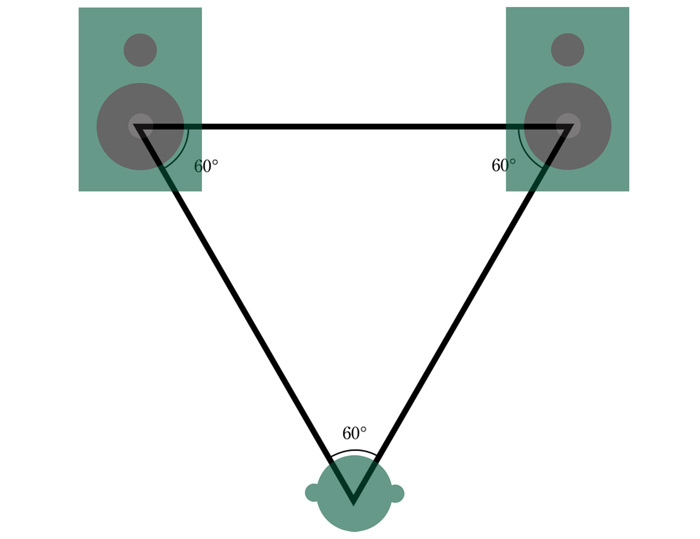
\includegraphics[scale=0.30]{figures/stereo.jpg}
	\caption {Configurazione stereo} 
	\label{fig:stereo}
	\end{figure}

Questo avviene sia per casse in aria libera che per cuffie. \\

Parlando dello stereo cominciamo a parlare di standard in quanto la configurazione prevede di creare un triangolo equilatero con ai vertici i due altoparlanti e l'ascoltatore, se non si segue questa direttiva non si avrà la giusta spazialità e collocazione spaziale dei suoni.\\

Questi descritti sono i metodi principali di riproduzione in cui si comincia ad intravedere un primo approccio di spazializzazione	 sonora, ora l'ascolto di musica si ferma generalmente qui alla riproduzione in una dimensione ma l'avvento dei film e dei cinema ha portato al concetto di audio in due dimensioni in particolare al surround.

\subsection{Audio in due dimensioni}

Per audio in due dimensioni si intende una riproduzione che pone l'ascoltatore al centro di un piano di diffusione in modo che si possano sentire suoni provenienti anche dai lati e da dietro; diverse sono le configurazioni possibili ma quelle che interessano a noi sono principalmente tre.\\

La più diffusa configurazione surround è sicuramente la \textbf{5.1} \footnote{dove la prima cifra sta per il numero di diffusori nel piano e la seconda cifra sta per il numero di LFE (canale audio dedicato al subwoofer)} usata principalmente dalla Dolby e dalla DTS per riproduzione di audio per film.


Questa configurazione, come spiega da specifica \cite{5.1}, è composta da un canale LFE per il subwoofer e di 5 canali distribuiti in 5 satelliti disposti rispettivamente a 0°, $\pm$30° e $\pm$110/120°\\

Una successiva configurazione è la \textbf{7.1} che riporta angoli di 0°, $\pm$30°, $\pm$90/110° e $\pm$135/150°

\begin{figure}[htbp]
	\centering
	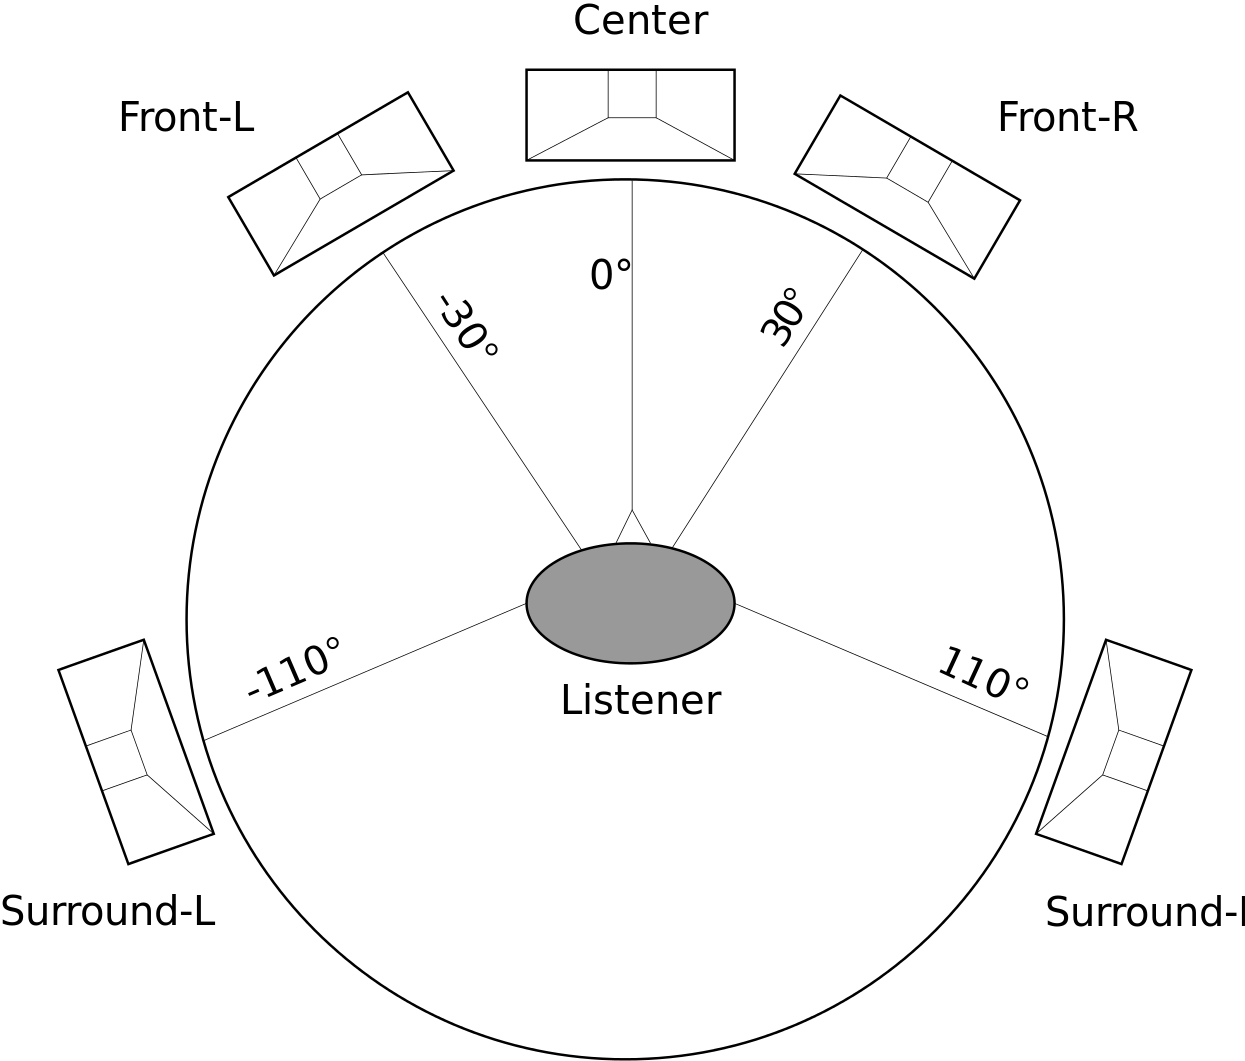
\includegraphics[scale=0.18]{figures/5-1.png}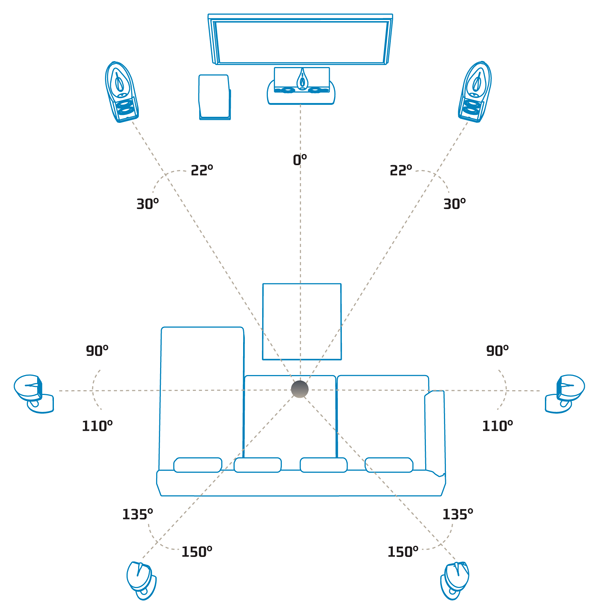
\includegraphics[scale=0.34]{figures/7-1.png}
	\caption {Configurazione 5.1 e 7.1} 
	\label{fig:5.1}
	\end{figure}
  

\section{Stream audio object-oriented}

Ora capito quali sono i principali standard di riproduzione andremo a spiegare come come queste configurazioni andranno pilotate, non ci interessa tanto il contenuto di ogni canale ma il fatto che: 

\begin{itemize}
\item nel più semplice dei casi ad ogni speaker sarà assegnato un canale audio differente (esempio Dolby Digital 5.1 dove ad ogni altoparlante è pilotato da un segnale discreto indipendente), si veda \cite{digital}.
\item nei casi più complessi ad ogni altoparlante sarà assegnato un mix di canali dato da una matrice di decodifica proprietaria (esempio si guardi il funzionamento del decoder Dolby Pro Logic), si veda \cite{prologic}.
\end{itemize}

Un'altra importante considerazione è il fatto che lo stesso stream che utilizzo in un sistema "di grado maggiore" per esempio un 5.1 posso "scalarlo in un sistema "di grado minore" esempio uno stereo, questo perchè essendo tutti questi degli standard è possibile fare un downgrade dello stream oppure un upgrade (solo però solto alcuni artifici" per essere adattato al sistema di riproduzione; allora viene da chiedersi perchè cambiare concenzione e approdare in uno stream object-oriented?\\

La domanda trova facile risposta nel fatto che questi giochi di upgrade o downgrade si possono fare solo su sistemi che hanno una certo grado di compatibilità (ad esempio i sistemi Dolby) e se questo avvenisse dovrei comunque prendere uno stream, codificarlo in uno stream diciamo "generale" e riadattarlo decodificandolo nello stream che piloterà la mia riproduzione.\\

Allora la domanda sorge spontanea, perchè non creare uno stream diciamo generale?

La Dolby laboratories ha già implementato una tecnologia che risponde in questa domanda, infatti nel suo ultimo brevetto \textbf{Dolby Atmos} (si veda documentazione \cite{atmos}) ha implementato nello stream di riproduzione anche una parte dedicata agli oggetti sonori, infatti oltre ad avere un tappeto sonoro dato dalla configurazione 7.1, la configurazione dolby atmos permette la creazione di 128 oggetti indipendenti nello spazio sonoro 3D che vengono riprodotti grazie anche all'ausilio di speaker posti al di sopra dell'ascoltatore, ma non ci soffermeremo troppo su questa configurazione, piuttosto spenderemo tempo a parlare di come Dolby é riuscita incanalare gli oggetti e la relativa informazione spaziale dentro questo stream.\\

Normalmente quando si crea un prodotto in fase di post-produzione si fa un down-mix del prodotto per passare dal contenuto dei singoli canali allo stream di riproduzione, per esempio chiudendo un mix in uno studio di registrazione classico miscelo i vari canali nello stream audio stereo con peso costituito dalla funzione di panpot deciso per ogni canale, questo succede anche in configurazioni più complicate come il 5.1 l'unica differenza è che panpot non sarà più in una dimensione ma in due\footnote{esiste una funzione di panpot standard per ogni configurazione di riproduzione}.\\

L'idea della Dolby invece è stata quella di fermarsi prima della fase di downmix (almeno per quanto riguarda il contenuto degli oggetti sonori) e di intraprendere una strada diversa:\\

Prima di tutto si devono preparare gli oggetti sonori esattamente come si vuole siano riprodotti, in secondo luogo si dispongono questi oggetti in uno spazio di riproduzione virtuale creato appositamente da un qualche software o plugin nel quale a ogni oggetto verrà assegnato un punto preciso nello spazio attraverso delle coordinate spaziali.

Questo sostanzialmente sta alla base dell'audio ad oggetti, nel prossimo capitolo vedremo come concretamente implementare questo nuovo procedimento.



\chapter{Spazilizzatore 3D e Format MDA}

In questo capitolo andremo a spiegare concretamente come possiamo creare questo stream audio ad oggetti e come in fase di post produzione posso spazializzare il mio contenuto sonoro.\\

Come accennato prima in fase di post-produzione non usiamo più il solito panner installato in banchi mixer o in sofware DAW in quanto essi sia che siano stereo o 5.1 o quello che vogliamo, non hanno una spazializzazione a oggetti quindi la cosa da fare è implementare un software apposito che, sotto forma di stand-alone o di plug-in, dia in uscita gli oggetti sonori con la loro relativa posizione (in realtà oltre che alla posizione bisognerà tener conto anche di altri paramentri come grandezza, volume ecc...).\\

Parlando fino ad ora di Dolby è plausibile che prenderemo come panner 3D e come format\footnote{per format intendo lo stesso concetto che in procedenza ho usato con la parola stream} quello proprietario di Dolby Atmos ma il fatto è che essendo questa tecnica di spazializzazione soggetta a brevetto, essa é diciamo chiusa a sole applicazioni che riguardano il mondo Dolby, altri marchi hanno prodotto format proprietari simili ma sempre vincolati al brevetto, format quali Auro3D per citarne uno.\\

Noi invece ricerchiamo qualcosa che sia un format open e libero in grado di adattarsi e a diventare uno standard; la \textbf{Digital Theater System DTS} (storica rivale di Dolby) anche lei interessata all'audio ad oggetti ha creato un format open che fa al caso nostro: questo si chiama \textbf{Multi-Dimesional Audio MDA}.\\

\section{Format MDA}

Si veda \cite{mda} per la documentazione riguardante questo paragrafo.\\

Il gioco che sta alla base di questo format è la scrittura di \textbf{metadati} contenenti gli attributi dell'oggetto sonoro da spazializzare, questo format essendo principalmente stato creato per il cinema avrà attributi che per la sola riproduzione musicale sono non necessari ma di questo ne parleremo dopo.\\

Questi attributi sono:
\begin{itemize}\label{aaa}
\item \textbf{Coordinate Spaziali}: sono un set di 3 valori che indicano la posizione dell'oggetto sonoro in relazione con la posizione dell'ascoltatore che avrà come valori la terna (0,0,0).\\

Come coordinate abbiamo l'asse $X$ posto di fianco all'ascoltatore, l'asse $Y$ posto di fronte e l'asse $Z$ posto verso l'alto, quindi definito un angolo di azimut $\theta$, un'angolo di elavazione $\phi$ e un raggio $\rho$
posso definire le coordinate polari come:

\begin{equation}
	\left\{\begin{matrix}
x=\rho sin(\theta) cos(\phi) \\
y=\rho cos(\theta) cos(\phi)\\
z=\rho sin(\phi)\\
\end{matrix}\right.
	\label{eq:coordinatepolari}
\end{equation}

\begin{figure}[htbp]
	\centering
	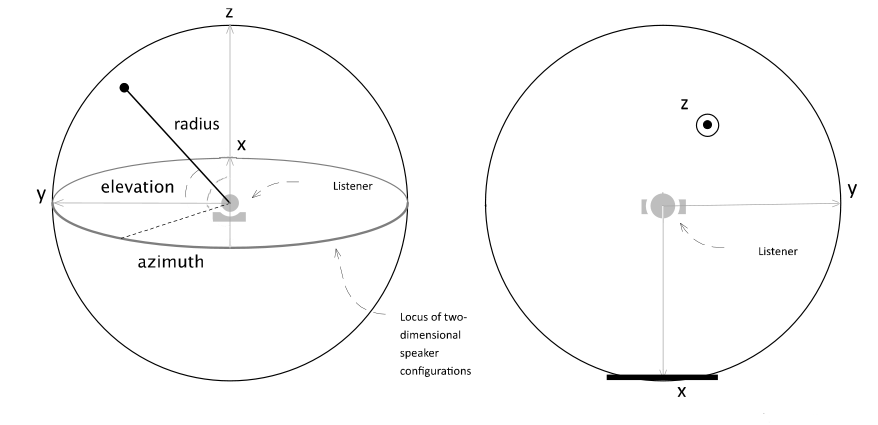
\includegraphics[scale=0.35]{figures/azimut.png}
	\caption {Coordinate spaziali} 
	\label{fig:coordinate}
	\end{figure}
	
\item \textbf{Identificativo oggetto sonoro}: scritto come URI é un numero (int) che identifica l'oggetto sonoro, sarebbe come un indirizzo.
\item \textbf{Gain}: è un valore che indica la quantità di segnale che deve avere l'oggetto sonoro.
\item \textbf{apertura}: scritta in gradi indicherebbe la grandezza dell'oggetto sonoro da ricreare(più l'oggetto è grande più gli altoparlanti posti marginalmente della sorgente fantasma si attivano, esempio se il valore è 180° allora si attiverebbero tutti i diffusori)
\item \textbf{divergenza}: anch'essa indicata in gradi quantifica la grandezza che deve avere l'oggetto sonoro ma solo sul piano orizzontale, un esempio più esplicativo si ha in figura \ref{fig:apertura}.
	
	\begin{figure}[htbp]
	\centering
	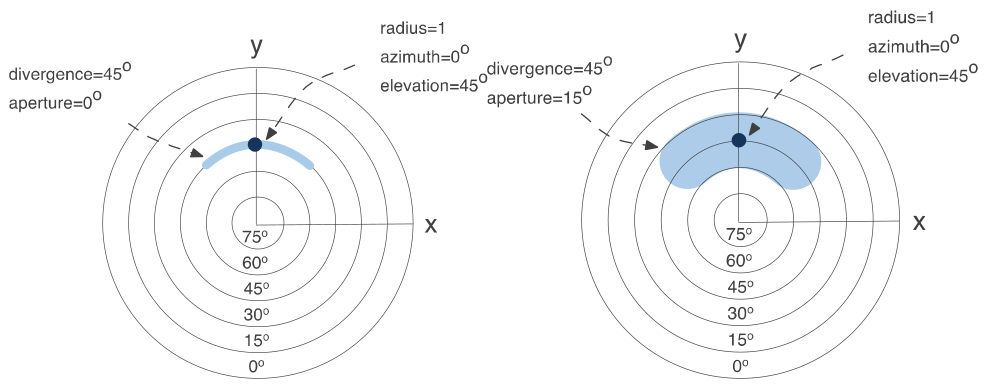
\includegraphics[scale=0.35]{figures/apertura.png}
	\caption {parametri di apertura e divergenza} 
	\label{fig:apertura}
	\end{figure}
	
	
\end{itemize}

queste sono i principali parametri scritti nei metadati che ci servono per la spazializzazione, abbiamo quindi un  oggetto sonoro e i suoi metadati ma è facile pensare che se l'oggetto si muove nello spazio o cambia dimensioni il contenuto dei suoi matadati cambia nel tempo, quindi il format racchiude in un nuovo oggetto chiamato "\textbf{Object-Fragment}" dove saranno segnati tutti metadati descritti sopra (che per tutto lo svolgimento temporale dell'object fragment rimarranno inalterati) con più l'aggiunta di alcuni parametri come l'\textbf{ID} (identificativo oggeto), e i sample dell'oggetto sonoro da riprodurre.\\

Sopra tutto poi c'è una timeline (figura \ref{fig:time}) che ha la funzione di richiamare gli object-fragment quando servono, essa è suddivisa in segmenti temporali che sono dati da $\dfrac{1}{f_c}$ dove $f_c$ è la frequenza di campionamento impostata per la totalità degli oggetti sonori, e dove a ogni segmento è associato una lista di ID che richiama oggetti da riprodurre, un'esempio esplicativo è dato dallo schema \ref{fig:object}.\\

\begin{figure}[htbp]
	\centering
	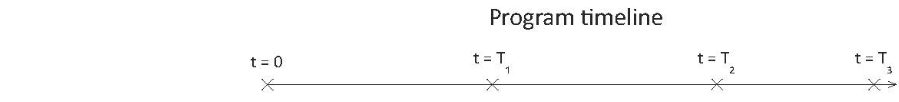
\includegraphics[scale=0.50]{figures/timeline.png}\\
	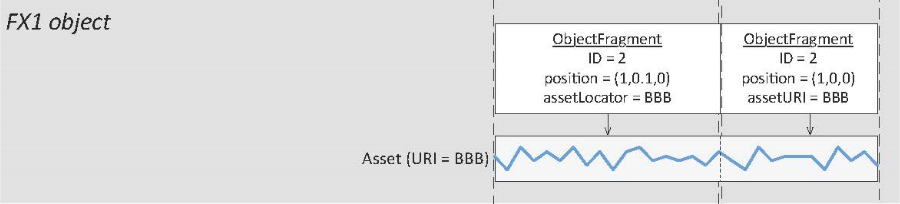
\includegraphics[scale=0.50]{figures/object1.png}\\
	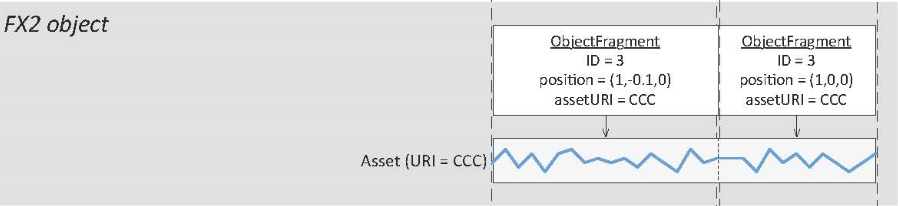
\includegraphics[scale=0.50]{figures/object2.png}\\
	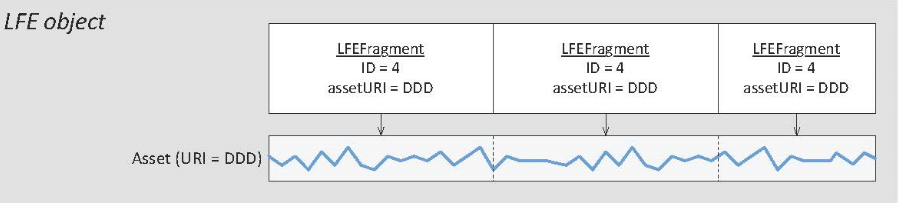
\includegraphics[scale=0.50]{figures/object3.png}
	\caption {Schema esplicativo funzionamento format MDA} 
	\label{fig:object}
	\end{figure}

\begin{figure}[htbp]
	\centering
	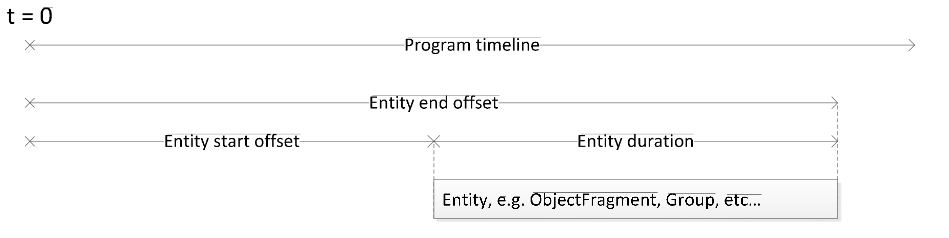
\includegraphics[scale=0.50]{figures/timeline2.png}
	
	\caption {azione di richiamo di un object-fragment} 
	\label{fig:time}
	\end{figure}

Da notare che è presente anche un LFE-Object in cui non è segnata la posizione, questo perchè data la natura omnidirezionale delle basse frequenze non avrebbe senso collocarle spazialmente e anche perchè solo il/i subwoofer sono in grado di riprodurre tali frequenze.

\subsection{format MDA per riproduzione audio}

Qui faccio una piccola annotazione personale che mi tornerà utile più avanti, nella maggior parte dei casi quando si fa musica in studio di registrazione è abbastanza difficile che abbiamo oggetti sonori in movimento e di dimensioni che variano nel tempo, quindi si potrebbe fare una piccola modifica al format in modo da alleggerire il succesivo rendering per creare fisicamente lo spazio sonoro.\\

Sostanzialmente abbiamo tre tipi di oggetti sonori in musica: oggetti fermi, oggetti che "balzano" tra due punti spaziali ed oggetti costituiti da effetti vari (il più importante per la spazializzazione è il riverbero e per questo ci occuperemo solo di questo).

tutti questi oggetti possono essere pensati come oggetti statici quindi che hanno coordinate spaziali e dimensioni fisse, in questo caso si potrebbe alleggerire il format in quanto non avrebbe più senso parlare di object-fragment (ricordiamo che gli attributi di spazializzazione cambiano allora si avranno diversi object-fragment, uno per ogni configurazione spaziale) in quanto per l'intera esecuzione del brano si avrebbe solo un object-fragment che fissa la posizione e la grandezza dell'oggetto, quindi si possono direttamente assegnare queste due ultime all'oggetto sonoro senza passare per ulteriori sottodivisioni.\\

per quanto riguarda gli oggetti statici questo trucco calza alla perfezione, per il riverbero per esempio basterà avere come oggetto il solo contenuto del brano riverberato e assegnarli una giusta divergenza e apertura; per quanto riguarda gli oggetti "balzanti" (come potrebbe essere per esempio un tremolo fatto con un pan-pot in una tastiera) basterà creare in fase di post-produzione due oggetti diversi che hanno lo stesso contenuto sonoro e che differiscono soltanto che l'intensità sonora $I'=\alpha I$ di un'oggetto corrisponderà a una intensità $I''=(1-\alpha) I$ del secondo oggetto (dove $I$ é l'intensità che dovrebbe avere originariamente l'oggetto).

\section{Spazializzatore 3D}

Precedentemente abbiamo visto come è costituito il format MDA ora non ci rimane di piegare produrre materiale compatibile con questo format.\\

Nel workflow di produzione di materiale audio 3D bisognerà fermarsi quindi prima del mixdown (sia che sia stereo, 5.1 ecc...) e bisognerà prendere un qualche software che sia in grado di sostituire il mio mixer e sostituirlo con uno 3D, diverse aziende stanno facendo software di questo tipo in quanto vogliono interfacciarsi a questo format ed in qualche modo creare un collegamente tra il loro format proprietario e l'MDA; per esempio la Dolby ha un panner 3D per Dolby Atmos mka che si interfaccia con l'MDA, anche la Auro Technologies ha adottato la stessa politica o in alternativa la casa Fairlight ha creato uno spazializzatore di nome 3DAW (secondo me molto interessante) che supporta anche l'MDA.\\

Detto questo ho ricercato uno spazializzatore adatto e la mi ascelta è ricaduta proprio sull'\textbf{MDA creator} proprietaria della DTS in quanto è la più intuitiva ela miglior scelta per integrazione (in quanto essa ha creato sia il panner che il format).

\begin{figure}[htbp]
	\centering
	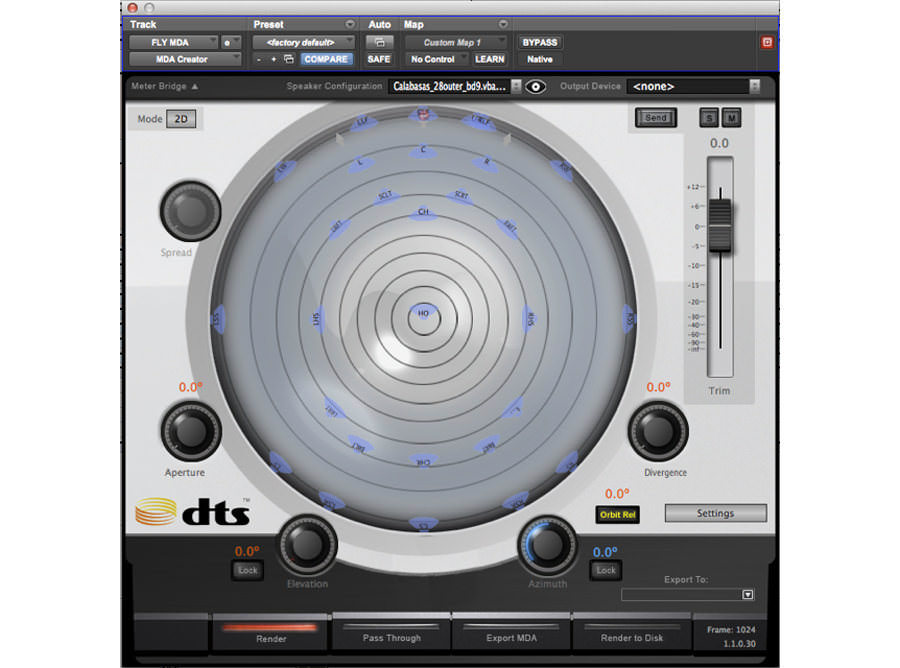
\includegraphics[scale=0.50]{figures/mdacreator.jpg}
	
	\caption {MDA Creator, DTS technology} 
	\label{fig:mdacreator}
	\end{figure}

Tutte le informazioni su MDA creator verranno prese dal suo manuale \cite{creator}.\\

questo plugin disponibile solo per Protools è di semplice comprensione, come da manuale bisogna mettere in insert in ogni traccia questo plugin (condizione necessaria è che tutte le tracce devono avere la stessa lunghezza), poi aprendo l'interfaccia del panner bisognerà posizionare ogni oggetto nel punto in cui si desidera e con divergenza e apertura voluta (si veda il paragrafo \ref{aaa} per sapere i parametri del format), logicamente questi parametri possono essere automatizzati per spostare e modificare l'oggetto nel tempo.

Inoltre si possono creare dei "Bed Object" che sarebbero oggetti i quali vengono direttamente codificati nel sistema di riproduzione scelto (esempio classico è la colonna sonora in 5.1 nei film) ai quali verranno sommati gli oggetti veri e propri del format e l'LFE-Object per gli effetti a bassa frequenza.\\

Una volta fatto questo l'MDA creator metterà a disposizione tre scelte di output, quella che interessa a noi è la modalità di esportazione con mda file: questa scelta ci porta alla creazione dei file \textbf{.map, .mix} e \textbf{.mda}, quest'ultimo è proprio il file contenente i metadati e gli oggetti sonori proposti in questo format.


\chapter{Decodifica format MDA per adattamento a varie configurazioni}

In questo capitolo parleremo di come invece da un format MDA posso passare a una configurazione di riproduzione usuale, mediante alcune tecniche quali il VBAP, il BINAURALE e la WFS.\\

\section{decodifica in VBAP}

Il \textbf{Vector Base Amplitude Panning VBAP} è una tecnica di spazializzazione che permette di localizzare una sorgente attraverso la differenza di intensità, mi spiego meglio:\\
uno dei due parametri con cui il nostro cervello discrimina la direzione di una sorgente è la IID (si veda \cite{iid}) che indica la differenza di intensità che le nostre orecchie devono percepire per far si che si percepiamo una sorgente fantasma in un punto dello spazio, quindi se riproduciamo un segnale coerente (cioè in fase fra gli altoparlanti) con minimo di due di essi e gli riproduciamo con intensità diverse, allora ci sembrerà di sentire il segnale proveniente da un punto previsto dalla IID.\\

Ora la cosa diventa abbastanza semplice in quanto se volgiamo ricreare una spazializzazione 2D basteranno due speaker, se invece vogliamo fare un 3D allora serviranno un minimo di 3 speaker posti a triangolo, configurazioni del genere esistono già e sono state ampiamente testate ed affinate,per tutta la documentazione riguardante il VBAP si faccia riferimento a \cite{vbap}.\\

E' d'obbligo affrontare un po di matematica per riuscire poi ad adattare il VBAP alle configurazioni esposte in \ref{metodi}, partiamo subito con il caso bidimensionale con 2 speaker affrontando la cosa direttamente con calcolo matriciale (all'inizio più difficile ma meglio generalizzabile per dopo).\\

Consideriamo un sistema fatto da due monitor, conoscendo la posizione della nostra sorgente virtuale (cosa che si adatta esattamente al nostro caso) l'unica cosa che non sappiamo sono i gain $g_1$ e $g_2$ da applicare ad ogni segnale che vanno rispettivamente alle due casse per ricostruire esattamente lo spazio sonoro, quindi definendo un sistema di riferimento cartesiano $\vec{X},\vec{Y}$ definirò come $l_1= {\left[ l_{11} \ l_{12} \right]}^T$ i vettori unitari che puntano verso i due altoparlanti e $p= {\left[ p_1 \ p_2 \right]}^T$ il vettore unitario che punta verso la sorgente virtuale.\\ 

Il trucco ora sta nel fatto che posso riscrivere il vettore $p$ in funzione del vettore contenente i due gain $g= \left[ g_1 \ g_2 \right]$ come:

\begin{equation}
p= g \cdot l = \left[g_1 \ g_2 \right] \left[l_1 \ l_2 \right]^T = g_1 l_1 + g_2 l_2
\label{eq:bbbb}
\end{equation}

In questo caso però possiamo ulteriormente compattare la scrittura in quanto:

\begin{equation}
p=g_1 {\left[ l_{11} \ l_{12} \right]}^T + g_2 {\left[ l_{21} \ l_{22} \right]}^T= \left[ g_1 \ g_2 \right] \left[\begin{matrix}
l_{11} & l_{12}\\ l_{21} & {l_22}
\end{matrix} \right]
\label{eq:cccc}
\end{equation}

ora trovando tutto in funzione $g$ abbiamo che:

\begin{equation}
\left[g_1 \ g_2\right] = \left[ p_1 \ p_2 \right]  {\left[\begin{matrix} 
l_{11} & l_{12}\\ l_{21} & l_{22}
\end{matrix} \right]}^{-1} \ \ \Rightarrow \ \ \ g=p^T {L_{12}}^{-1}
\label{eq:dddd}
\end{equation}

Logicamente assumo che la matrice $L_{12}$ ammetta l'inversa, fatto questo mi ritrovo con un'equazione a due incognite quindo devo trovare un qualcosa che leghi $g_1$ $g_2$ e in nostro aiuto viene la formula studiata da Blumlein e riproposta da Bauer che assieme alla formula \ref{eq:cccc} diventa:

\begin{equation}
\left\{ \begin{matrix}
\dfrac{tg (\phi)}{tg(\phi_0)}= \dfrac{g_1 - g_2}{g_1 + g_2} \\
\left[ g_1 \ g_2\right] = \left[ p_1 \ p_2 \right]  {\left[ \begin{matrix} 
l_{11} & l_{12}\\ l_{21} & l_{22}
\end{matrix} \right]}^{-1}
\end{matrix}\right.
\label{eq:eeee}
\end{equation}


\chapter{Metodo Wave Field Syntesis}

Il metodo Wave Field Syntesis è un metodo diverso dai precedenti illustrati in quanto non si avvale della psicoacustica per "ingannare" la nostra mente e farci credere che stiamo ascoltando qualcosa che realmente non c'è, ma questa tecnica permette di ricreare fisicamente il fronte d'onda e quindi l'informazione sonora distribuita nello spazio acustico come se la sorgente che si vuole creare sia realmente collocata nel punto che vogliamo, per questo, forse anche impropriamente, catalogherò questo metodo come \textbf{AUDIO 3D}.\\

\section{Principio fisico alla base e algoritmo di implementazione}

Per riuscire a capire in fondo cosa sta alla base di questa tecnica bisognerà spiegare due semplici principi di meccanica ondulatoria: 

\begin{itemize}

\item \textbf{Principio di Huygens-Fresnel}: consideriamo una qualsiasi onda che abbia un fronte d'onda arbitrario, questa legge afferma che ogni punto del fronte d'onda in questione può essere visto come un'infinità di sorgenti secondarie puntiformi che generano un'infinità di fronti d'onda secondari in accordo in fase e in ampiezza e che sommando la totalità di questi ultimi si può ricostruire il fronte d'onda originale.



\begin{figure}[htbp]
	\centering
	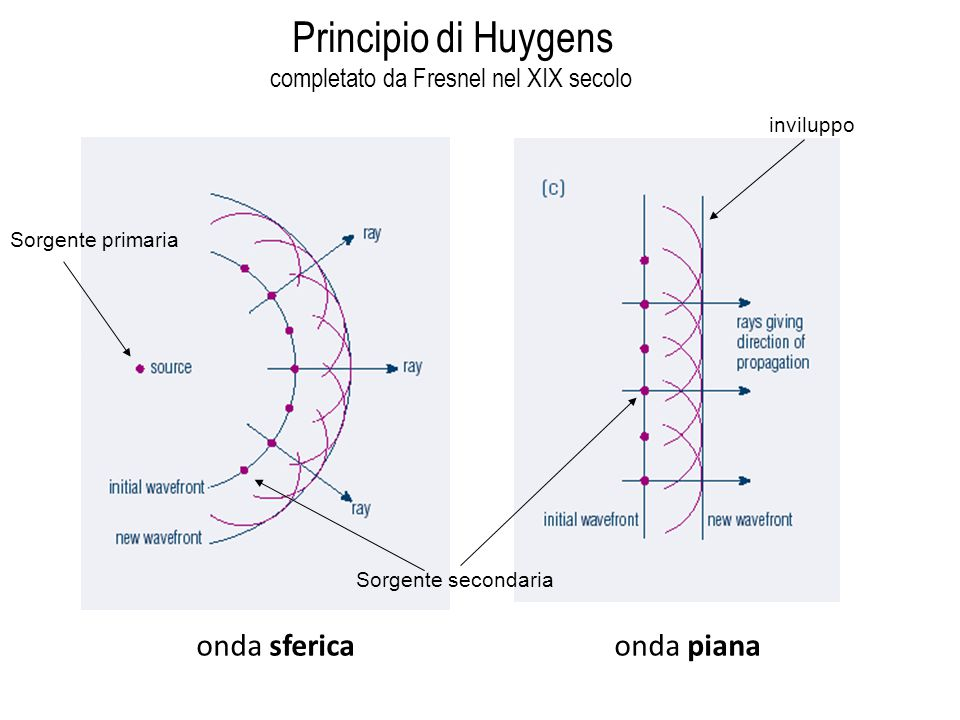
\includegraphics[scale=0.35]{figures/huygens.jpg}
	\caption {Principio di Huygens-Fresnel} 
	\label{fig:huygens}
	\end{figure}

\item \textbf{Principio di Rayleigh}: questo principio riguarda la diffrazione in quanto se un fronte d'onda colpisce una fenditura di dimensioni paragonabili alla sua lunghezza d'onda, esso verrà ritrasmesso al di la della fenditura come se fosse una sorgente puntiforme.

\end{itemize}

Il salto concettuale ora è breve in quanto se una sorgente acustica reale emette un fronte d'onda ed esso impatta in una serie di fenditure disposte spazialmente in un modo preciso, il fronte d'onda passerà al di ognuna delle fenditure (principio di Rayleigh) e la somma della totalità dei fronti d'onda secondari ricreerà esattamente il fronte d'onda originale.

Ora l'unica cosa che è rimasta da fare è sostituire ogni fenditura con un altoparlante e far riprodurre ad esso un  segnale preciso che combinato con i segnali degli altri altoparlanti ricreerà fedelmente (almeno a livello concettuale) lo spazio sonoro che vogliamo ottenere

\begin{figure}[htbp]
	\centering
	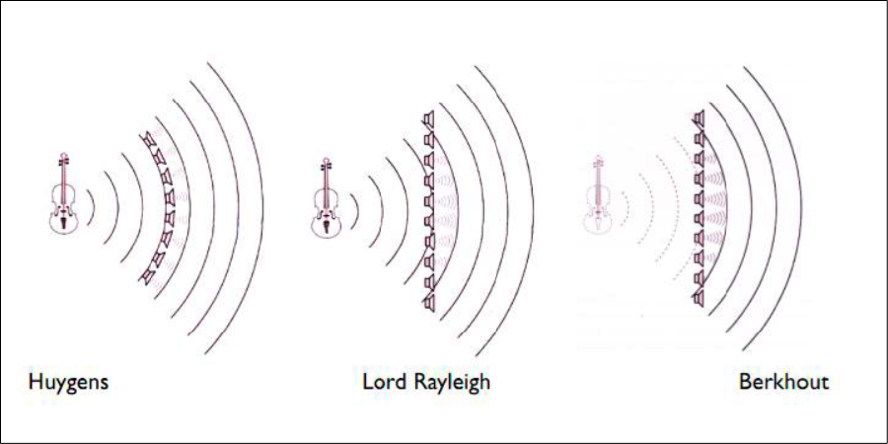
\includegraphics[scale=0.55]{figures/wfs.png}
	\caption {Salti concettuali della WFS} 
	\label{fig:wfs}
	\end{figure}
	

Ora le questioni che ci vengono naturali sono come e con quale segnale pilotare ogni altoparlante; le risposte possono essere molteplici ma tutte devono tener conto della geometria di progettazione del nostro sistema WFS, prendiamo uno dei casi più semplici.\\






\begin{thebibliography}{}

\bibitem{wikihuygens} \textit{https://en.wikipedia.org/wiki/Huygens-Fresnel\_principle}
\bibitem{5.1} \textit{https://www.itu.int/dms\_pubrec/itu-r/rec/bs/R-REC-BS.775-3-201208-I!!PDF-E.pdf}
\bibitem{digital} \textit{https://it.wikipedia.org/wiki/Dolby\_Digital}
\bibitem{prologic} \textit{https://it.wikipedia.org/wiki/Dolby\_Surround\_Pro\_Logic}
\bibitem{atmos} \textit{https://www.dolby.com/us/en/technologies/dolby-atmos/dolby-atmos-next-generation-audio-for-cinema-white-paper.pdf}
\bibitem{mda}\textit{http://www.etsi.org/deliver/etsi\_ts/103200\_103299/103223/01.01.01\_60/ts\_103223v010101p.pdf}
\bibitem{creator}\textit{//digitalcommons.calpoly.edu/cgi/viewcontent.cgi?article=1049}\&\textit{context=laessp}
\bibitem{iid} \textit{https://en.wikipedia.org/wiki/Sound\_localization\#ITD\_and\_IID}
\bibitem{vbap} \textit{http://lib.tkk.fi/Diss/2001/isbn9512255324/article1.pdf}
\end{thebibliography}
\addcontentsline{toc} {chapter}{Bibliografia}


\end{document}

